% Inputs and outputs of a streamPAMI algorithm.
% Compile: pdflatex inputOutputStreamPAMI.tex
\documentclass[tikz,border=8pt]{standalone}
\usetikzlibrary{positioning,arrows.meta,calc}

\definecolor{boxblue}{HTML}{2E5E7E}
\definecolor{srcpurple}{HTML}{6B3FA0}
\definecolor{newgreen}{HTML}{2E7D32}

\begin{document}
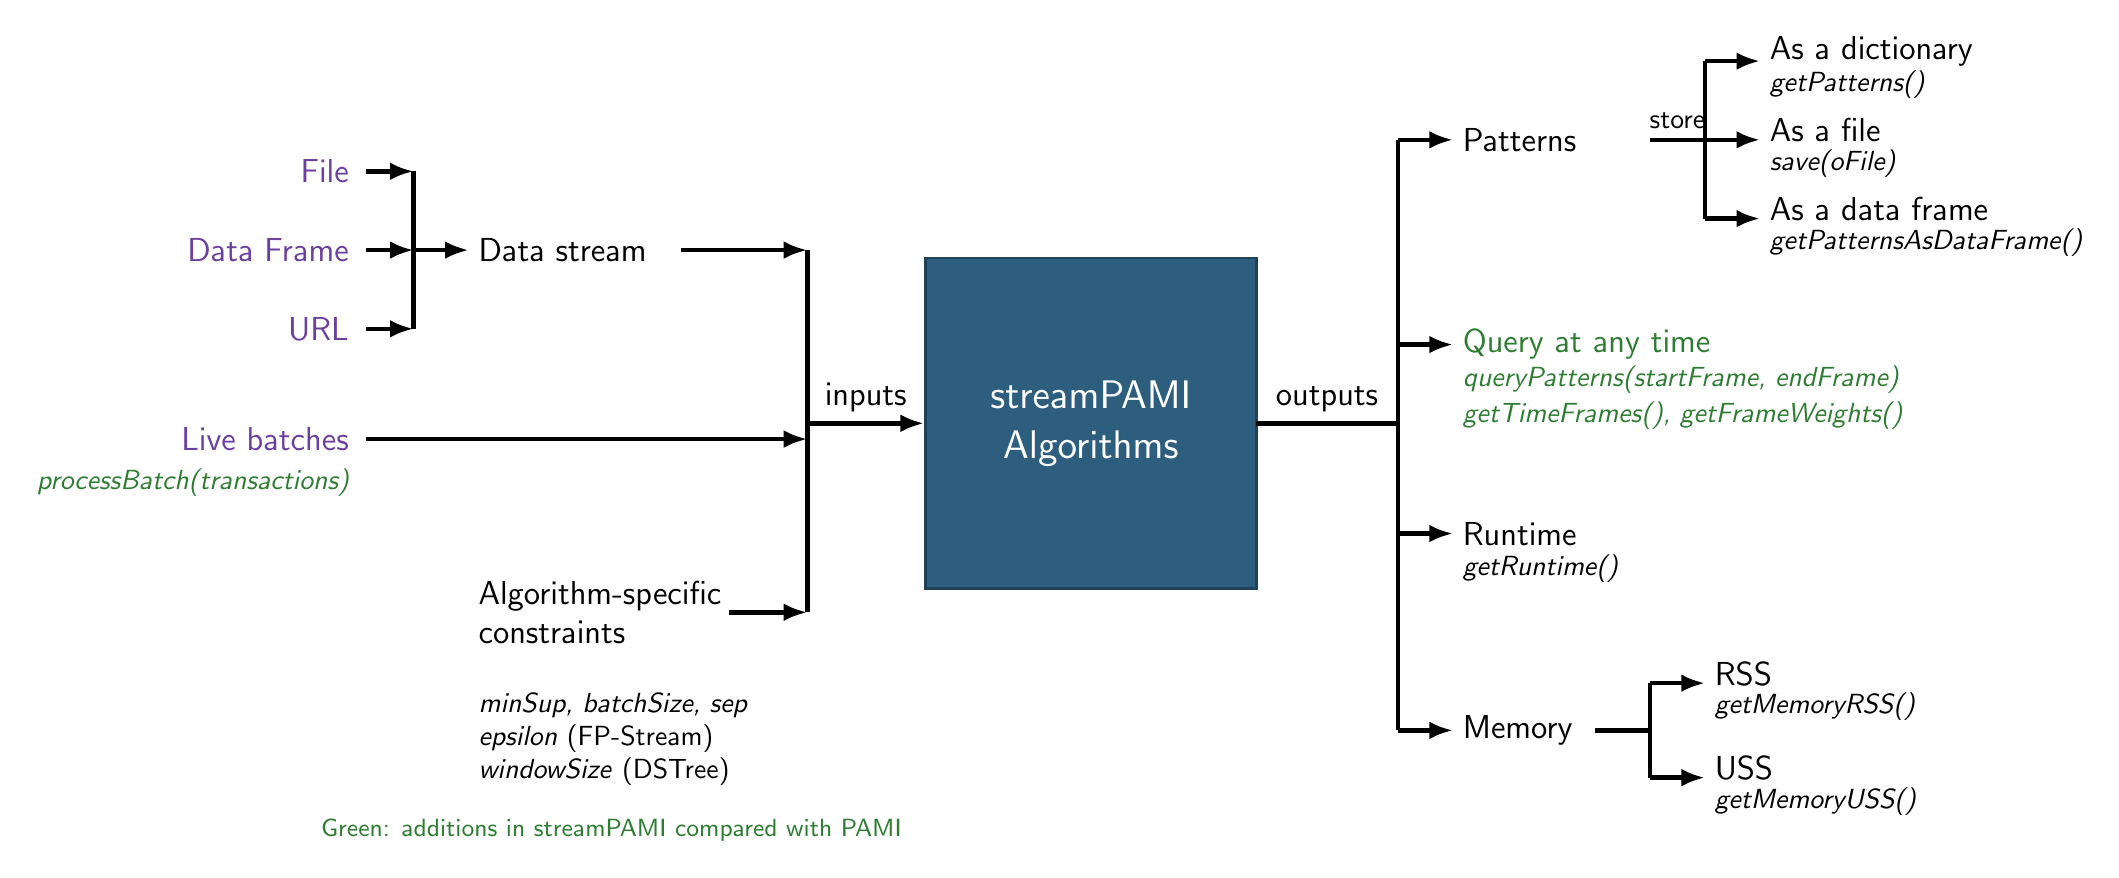
\begin{tikzpicture}[
    font=\sffamily,
    >={Latex[length=3mm]},
    line/.style={line width=1.6pt},
    arr/.style={line, ->},
    lbl/.style={font=\sffamily\large, align=left},
    src/.style={font=\sffamily\large, text=srcpurple},
    meth/.style={font=\sffamily\itshape\normalsize},
]

% ---------------- central box ----------------
\node[draw=boxblue!70!black, fill=boxblue, text=white, minimum width=4.2cm,
      minimum height=4.2cm, align=center, font=\sffamily\Large, line width=1pt]
      (algo) at (0,0) {streamPAMI\\Algorithms};

% ---------------- inputs ----------------
% Data sources
\node[src, anchor=east] (file) at (-9.3, 3.2) {File};
\node[src, anchor=east] (df)   at (-9.3, 2.2) {Data Frame};
\node[src, anchor=east] (url)  at (-9.3, 1.2) {URL};
\draw[line] (-8.6,3.2) -- (-8.6,1.2);
\foreach \y in {3.2,2.2,1.2} \draw[arr] (-9.2,\y) -- (-8.6,\y);
\node[lbl, anchor=west] (data) at (-7.9, 2.2) {Data stream};
\draw[arr] (-8.6,2.2) -- (data.west);

% Live batches
\node[src, anchor=east, align=right] (live) at (-9.3, -0.2) {Live batches};
\node[meth, anchor=north east, text=newgreen] at (-9.3, -0.45) {processBatch(transactions)};


% Constraints
\node[lbl, anchor=west] (cons) at (-7.9, -2.4) {Algorithm-specific\\constraints};
\node[meth, anchor=north west, align=left] at (-7.9, -3.3)
      {minSup, batchSize, sep\\epsilon \textup{(FP-Stream)}\\windowSize \textup{(DSTree)}};

% Merge into "inputs"
\draw[line] (-3.6,2.2) -- (-3.6,-2.4);
\draw[arr] (-5.2,2.2) -- (-3.6,2.2);
\draw[arr] (-9.2,-0.2) -- (-3.6,-0.2);
\draw[arr] (-4.6,-2.4) -- (-3.6,-2.4);
\draw[arr] (-3.6,0) -- (algo.west) node[midway, above, font=\sffamily\large] {inputs};

% ---------------- outputs ----------------
\draw[line] (2.1,0) -- (3.9,0) node[midway, above, font=\sffamily\large] {outputs};
\draw[line] (3.9,3.6) -- (3.9,-3.9);

% Patterns
\node[lbl, anchor=west] (pat) at (4.6, 3.6) {Patterns};
\draw[arr] (3.9,3.6) -- (pat.west);
\draw[line] (7.1,3.6) -- (7.8,3.6) node[midway, above, font=\sffamily] {store};
\draw[line] (7.8,4.6) -- (7.8,2.6);
\foreach \y/\t/\m in {4.6/As a dictionary/getPatterns(), 3.6/As a file/save(oFile), 2.6/As a data frame/getPatternsAsDataFrame()} {
  \draw[arr] (7.8,\y) -- (8.5,\y);
  \node[lbl, anchor=west] at (8.5,\y+0.12) {\t};
  \node[meth, anchor=west] at (8.5,\y-0.3) {\m};
}

% Query at any time (new in streamPAMI)
\node[lbl, anchor=west, text=newgreen] (qry) at (4.6, 1.0) {Query at any time};
\draw[arr] (3.9,1.0) -- (qry.west);
\node[meth, anchor=west, text=newgreen] at (4.6, 0.55) {queryPatterns(startFrame, endFrame)};
\node[meth, anchor=west, text=newgreen] at (4.6, 0.10) {getTimeFrames(), getFrameWeights()};

% Runtime
\node[lbl, anchor=west] (rt) at (4.6, -1.4) {Runtime};
\draw[arr] (3.9,-1.4) -- (rt.west);
\node[meth, anchor=west] at (4.6, -1.85) {getRuntime()};

% Memory
\node[lbl, anchor=west] (mem) at (4.6, -3.9) {Memory};
\draw[arr] (3.9,-3.9) -- (mem.west);
\draw[line] (6.4,-3.9) -- (7.1,-3.9);
\draw[line] (7.1,-3.3) -- (7.1,-4.5);
\foreach \y/\t/\m in {-3.3/RSS/getMemoryRSS(), -4.5/USS/getMemoryUSS()} {
  \draw[arr] (7.1,\y) -- (7.8,\y);
  \node[lbl, anchor=west] at (7.8,\y+0.12) {\t};
  \node[meth, anchor=west] at (7.8,\y-0.3) {\m};
}

% Legend for the green additions
\node[font=\sffamily\small, text=newgreen, anchor=north west] at (-9.9,-4.9)
     {Green: additions in streamPAMI compared with PAMI};
\end{tikzpicture}
\end{document}
